
\documentclass[conference]{acmsiggraph}

\TOGonlineid{45678}
\TOGvolume{0}
\TOGnumber{0}
\TOGarticleDOI{1111111.2222222}
\TOGprojectURL{}
\TOGvideoURL{}
\TOGdataURL{}
\TOGcodeURL{}

\title{Real-time shader-based rendering of grass}

\author {Kin Liu\\Manuel Reinfurt}
\pdfauthor{Kin Liu}

\keywords{radiosity, global illumination, constant time}

\begin{document}

\teaser{
  \frame{\includegraphics[height=1.5in]{images/final_result}}
  \caption{End result}
}

\maketitle

\begin{abstract}

Grass has always been an important factor when it comes to simulating realistic nature scenes. However, due to the sheer amount of individual grass blades and the need to animate them, it is very difficult to implement in real time applications. This paper tries to give an overview of the existing techniques that are used to render grass. It then goes in-depth about using the geometry shader to generate and render grass effectively in real time. Basics like grass vertex generation are explained, as well as animation using a simulated wind field. To conclude, the technique is being benchmarked as well as being looked at in terms of shortcomings and further improvements.

\end{abstract}

\TOGlinkslist

%% Required for all content. 

\copyrightspace

\section{Introduction}

Grass has always been an important factor when it comes to simulate realistic nature scenes. However, due to the sheer amount of individual grass blades and the need to animate them, it is very difficult to implement in real time applications. This paper tries to give an overview of the several techniques that are used in state of the art applications, as well as discussing a geometry-shader based approach in detail.

\section{Related Work}

There are different techniques on how to efficiently and realistically render grass in real time applications. In games, grass is usually simulated by rendering billboards that are laid our in a certain pattern. Animation can be done per vertex, per grass blade or even per cluster. A famous method has been described in GPU Gems 1. While this is a very simple approach that has been used in games for a long time since processing and graphics power is needed elsewhere, it does not yield stunning visuals.

Since DirectX 10, GPUs have been extended with a new shader pipeline - the geometry shader. Using the geometry shader, it is possible to generate grass blades directly on the GPU. This eliminates the CPU as a bottleneck and provides enough power for much more detailed simulations. This paper is based on this approach and combines the work of Eddie Lee \cite{EddieLee}, Kevin Boulanger \cite{KevinBoulanger} and Markus R. Tillmann.  \cite{Tillmann}

 \begin{figure}[ht]
   \centering
   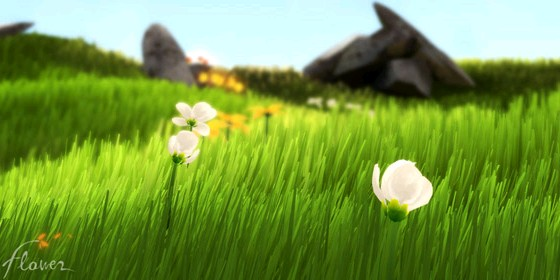
\includegraphics[width=2.5in]{images/flower_game}
   \caption{Game "Flower" for PlayStation 3} \cite{Flower} \footnote{URL: thatgamecompany.com/games/flower/}
 \end{figure}    
 
The game "Flower", which was released for PlayStation 3, uses this method to render all of its grass. This shows that the approach can be used in real time applications with much success. While the scenes in "Flower" were not really complex and mostly consisted of grass only, the hardware is already very old for todays standards - leaving enough power for more complex scenes which include grass simulation.

\subsection{The Method}
The basic idea is to layout the grass field on the CPU by specifying the root points. This way, the CPU only has to send the position of each single root to the GPU - all other work is done exclusively on the GPU. In order to organize the root points, grass patches are created. Each patch has a certain number of root points and can be controlled individually. The grass patches together then 
make up the grass grid - which is the grass field.

 \begin{figure}[ht]
   \centering
   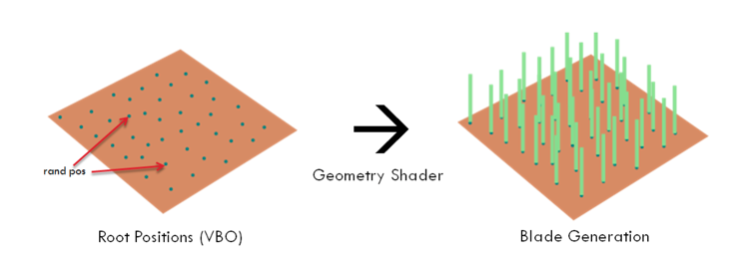
\includegraphics[width=3.5in]{images/grass_grid}
   \caption{Grass grid visualized} \cite{EddieLee}
 \end{figure}

The grass grid is generated by laying down root points as can be seen in Figure {?}. First, a grid of patches is created and each patch generates its own root points. Using a density map {Figure ?} that is equal the size of the terrain height map, local density spots can be adjusted to control the distribution of the grass. All root points are pushed into a single vertex buffer object and can be, in theory, rendered with a single draw call. However, the patches are used to achieve several things:

\begin{description}
  \item[Culling] \hfill \\
  A single patch can be visualized by a bounding box, which can then be easily checked against the view frusrum to cull patches outside of it. It is important to take the grass animation into account when creating the bounding box - otherwise grass could be culled when moving into the frustum.
   \begin{figure}[ht]
   \centering
   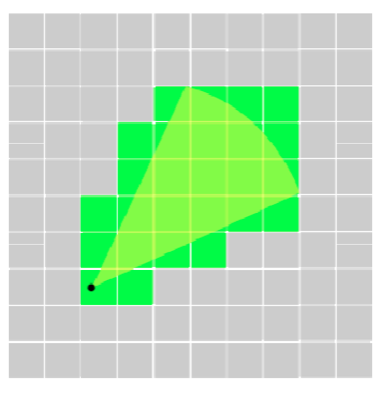
\includegraphics[width=2.0in]{images/culling}
   \caption{Culling of patches outside the frustum} \cite{EddieLee}
 \end{figure}    
  
  \item[Level of detail] \hfill \\
  The distance from the camera to the mid point of a patch can be calculated and used to set the level of detail. This saves a few instructions as level of detail does not have to be calculated within the geometry shader, thus making it possible to use geometry shaders that are pre-compiled with a static vertex count, which will improve performance.

 \begin{figure}[ht]
   \centering
   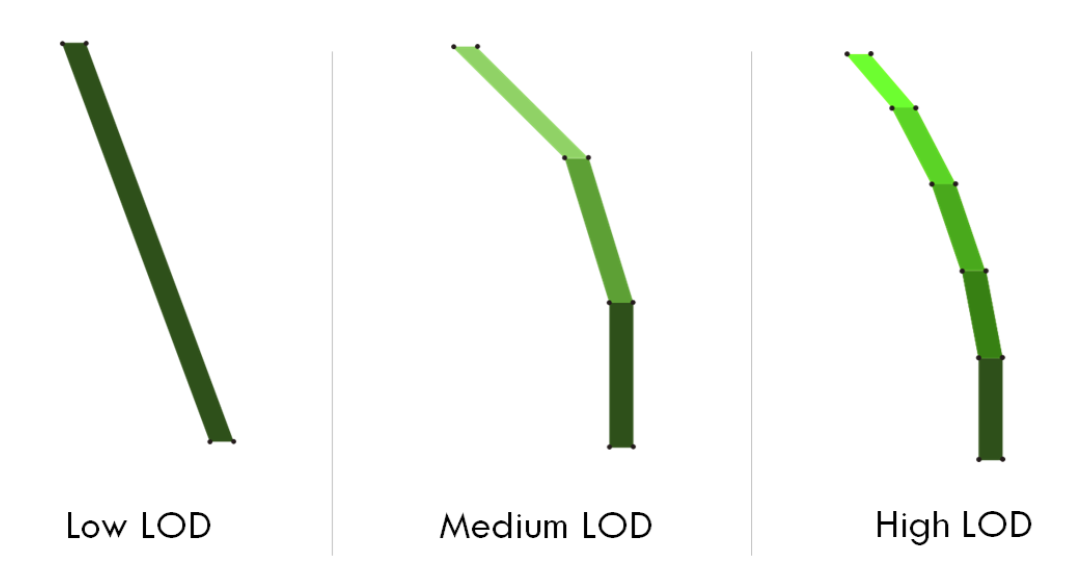
\includegraphics[width=3.0in]{images/lod}
   \caption{Vertices for level of detail} \cite{EddieLee}
 \end{figure}  
  
  \item[Further individualization] \hfill \\
	It's possible to pass options into the shaders for rendering a patch, which can be used for wind animation, grass height or any other property of the grass.
\end{description}

While rendering the patches individually adds overhead compared to doing a single draw call for the vertex buffer object, the performance improvements using the methods above, as well as further individiualization of the scene, more than make up for it.

\subsection{Generating the blade}
The geometry shader needs to be able to generate grass blades with a different level of detail. Instead of writing separate geometry shaders, we decided to write one geometry shader that prodecurally generates the blade. When generating the blade, we want to concentrate the vertices on the top half of the blade to have a smooth animation later on. It is also needed to calculate the UV-coordinate, normals and rotation, as well as vertex displacement for wind, which is described in chapter 4.

 \begin{figure}[ht]
   \centering
   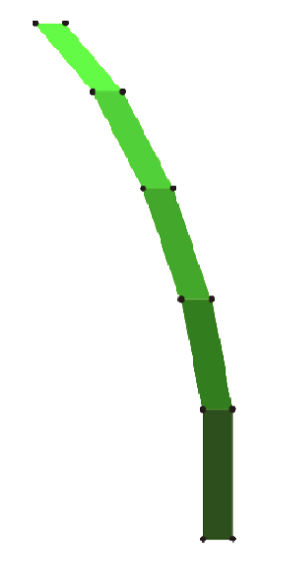
\includegraphics[width=0.75in]{images/grass_blade_vertices}
   \caption{Vertices of the grass blade} \cite{EddieLee}
 \end{figure}

To generate the blade, we start from the bottom and always generate a pair of vertices - one for the left and one for the right. We then move upwards, which is called a "step". In each step, we have to recalculate important variables. For example, we have to calculate the normal, UV-coordinate and lighting vectors (vertex to camera, vertex to light). However, it is not good enough to linearly go up and increase the values. Instead, we distribute the vertices so that there are more vertices on the top of the blade. Since the top of the blade is the part that will move the most (using wind animation), higher detail is much appreciated. Of course, this also means that other values, like normals, have to be adjusted as well. Our distribution is based on the simple function below.

\begin{equation}
y = x^2
\end{equation}

It's important to point out that our y values are ranging from 0 to 1 and thus we accumulate a lot of vertices on the top of the blade. Since we have a TriangleStrip, we iterate through each vertex and connect the next 3 vertices - until we hit the last vertex.

As a sidenote, an easy way to simulate good lighting is by artificially creating normals pointing downwards at the root of the blade, and as you go to the higher vertices, the normal can start to point upwards. This way, blades will be darker at the bottom and brighter at the top.

\subsection{Pipeline}
To summarize, this is a list of important components in our project and their respective job.
\begin{description}
  \item[CPU] \hfill \\
  The CPU will generate the root points out of the density map and create a single vertex buffer, that contains all roots. It will also slice the full grass grid into smaller patches, which can be controlled through constant buffers on the GPU.
  
  Since we also have static terrain, the root points will already contain the correct displaced Y position. Additional improvements like culling will also be done on the CPU.
  \item[Vertex shader] \hfill \\
  The vertex shader is, in essence, a pass-through shader.
  \item[Geometry shader] \hfill \\
  All the hard work is done in the geometry shader. Since the geometry shader gets a single point as an input, it's job is to create a grass blade with a specified number of vertices. The geometry shader will also take care of calculating normals, level of detail, and animation.
  \item[Pixel shader] \hfill \\
  To calculate the color, we use the basic Phong BDRF, combined with a texture and a randomized tint.
\end{description}

\subsection{Flickering}
A very prevalent problem while implementing this approach was flickering. Due to the high amount of very thin grass blades, blades were fighting for pixels and a lot of aliasing and flickering could be seen. In order to minimize this effect, several techniques were used:

\begin{description}
  \item[Grass blade proportions] \hfill \\
  Since grass blades far in the distant can not really be distinguished from each other due to having only a few pixels to be displayed, it is possible to increase the width of the grass blades. This way, less blades will be fighting for the pixel - having a clear winner in terms of which color to display, leaves less flickering.
  \item[Density Control] \hfill \\
  Since the goal is to minimize the amount of blades fighting for the pixels, the grass density (number of root points in a patch) can be adjusted depending on the distance to the camera. Combined with the grass blade proportions, this leaves very few grass blades that will fill the space in the distance. However, it should be noted that this approach can lead to grass blades "popping" in and out of the user's view. \cite{KevinBoulanger}
  \item[Downsampling] \hfill \\
  The simplest approach is to increase the render target resolution. Rendering the scene at 4k or 8k resolutions and then downsampling it to Full-HD leaves a stunningly clear and flicker-free image behind. While being simple to implement and having very good results, it has the highest performance cost. 
\end{description}

\subsection{Randomization}

The scene looks very artificial if the grass is laid out with exact distances, when each grass blade has the same tint, height or width. However, it is fairly difficult to generate random numbers on the GPU, which is why we have to use certain tricks to have fairly random grass properties. When laying out the root points, we can generate random positions using the CPU.

 \begin{figure}[ht]
   \centering
   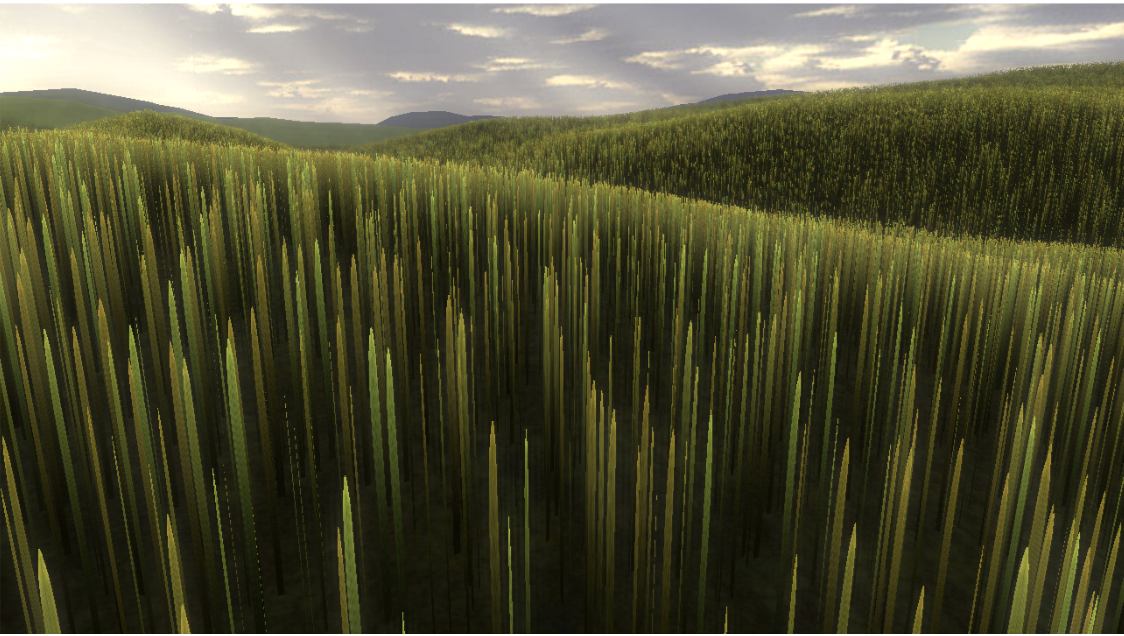
\includegraphics[width=3.5in]{images/no_randomness}
   \caption{Scene without randomness: Seems artificial} \cite{EddieLee}
 \end{figure}

Since these root points are given to the geometry shader, and we kow that these positions are random, we can generate a random number between -1 and 1 using the following equation.

\begin{equation}
r = sin(\frac{\pi}2 * frac(root.x) + \frac{\pi}2 * frac(root.z))
\end{equation}

Using this randomized value, several grass properties can be influenced. Some of those are: width, height, color tint, rotation, wind effect.

\section{Terrain}
To make the grass feel more like it sits in an environment instead of just floating in 3D-space, a terrain is created using a heightmap.

\subsection{Heightmap}
The heightmap is an image 8-Bit greyscale image containing the height values of the terrain. A mesh is generated, which has the same amount of vertices as the pixels of the heightmap image. The grey values, ranging from 0 to 255, are used to determine the height of the mesh at the corresponding position. When using the true grey values of the heightmap, the resulting terrain has very steep hills and valleys. To flatten the terrain, the heightvalues are divided by a certain factor

The heightmap is generated by using the cloud-filter function of Photoshop, which uses perlin noise to generate a noise texture. These noise textures have smoothed out grey values, which makes them well suited for creating mountain-like terrains. These textures are also seamless, which can be used for tiling an creating endless terrains.

 \begin{figure}[ht]
   \centering
   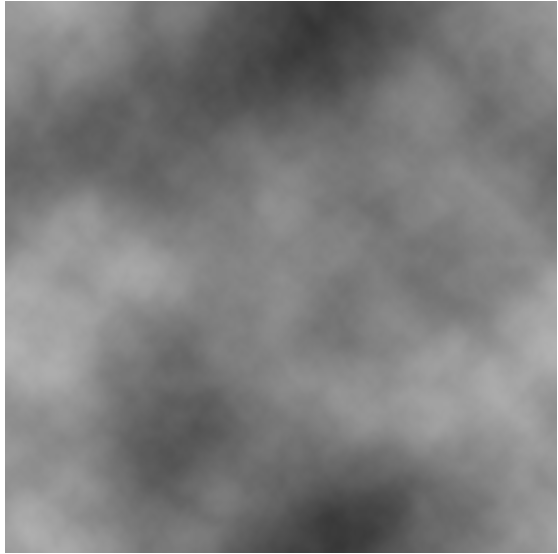
\includegraphics[width=1.5in]{images/heightmap}
   \caption{Noise texture created using cloud-filter}
 \end{figure}

\subsection{Mesh generation}
The mesh created for the terrain is basically a grid which consists of triangles, the height of the vertices are then offsetted by the values found in the heightmap.

 \begin{figure}[ht]
   \centering
   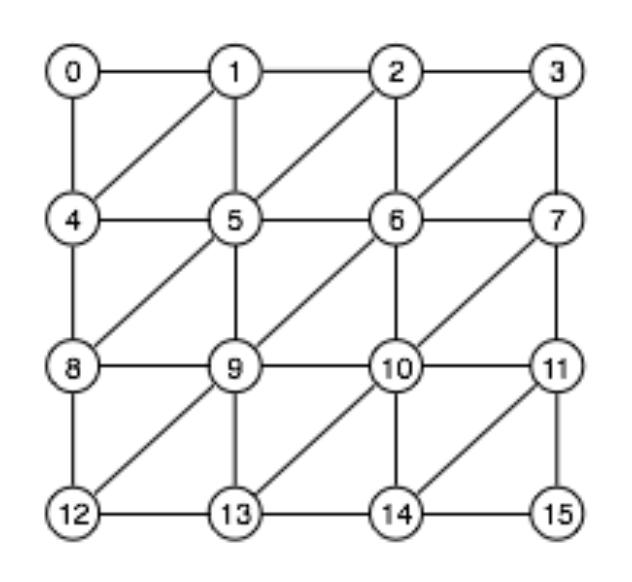
\includegraphics[width=1.5in]{images/terrain_grid}
   \caption{Grid made of triangles}\cite{TerrainGrid}
 \end{figure}

To create this sort of mesh, the indices have to be calculated in order for triangles to be generated properly. Starting from the vertice with index 0, which represents the upper-left corner of the first quad, the other corners (vertices 1, 4 and 5) are calculated. The indices for the cornes are calculated by using the following formulas:

\begin{description}
  \item[Upper Right] \hfill \\
  By adding 1 to the first indice, the index of the upper-right corner can be found:
\begin{equation}
UpperRight = UpperLeft + 1
\end{equation}
  \item[Lower Left] \hfill \\
  To find the lower-left corner, the total width of the mesh is added to the upper-left corner. In Figure 2, this would be 4, when using a heightmap it would be the width of the heightmap image:
\begin{equation}
LowerLeft = UpperLeft + width
\end{equation}
  \item[Lower Right] \hfill \\
The lower-right corner is found by adding 1 to the lower-left corner:
\begin{equation}
LowerRight = LowerLeft + 1
\end{equation}

By using these formulas, the first resulting indices are 0, 1, 4 and 5. Two triangles can now be created, by connecting UpperLeft, UpperRight and Lowerleft as well as LowerLeft, UpperRight and LowerRight. This would specify the triangles [0, 1 ,4] and [4, 1, 5]. This can be repeated for all vertices, thus creating a grid made of triangles. 
  
\end{description}

\subsection{Normal calculation}
The generated terrain is still missing something important, which is proper shading. Without the correct normals, the mesh just looks a sillouhette of a terrain when viewed in solid shading-mode. To achieve a smooth-shaded look, the vertex normals have to be calculated. This might seem counterintuitive, since vertices don’t actually have a normalvector. In practice, when having calculated the vertex normals, the rasterizer interpolates the values, hence creating a smooth-shaded look. A simple method of calculating vertex normals which yields reasonable results is by using averaged normals. First the vertex normals, which are identical to the surface normals, are calculated by  taking the cross product  of two edges of a triangle. The averaged normals are  then calculated by taking the normal of one vertex and adding the normals of adjacent vertices. The resulting normal is then normalized.\cite{Rasterizer}

 \begin{figure}[ht]
   \centering
   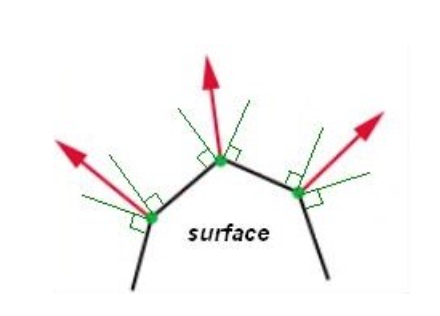
\includegraphics[width=1.5in]{images/terrain_normals}
   \caption{Vertex normal vectors (green), Averaged normals (red)} \cite{TerrainNormals}
 \end{figure}

\subsection{Grass displacement}
Placing the grass blades on the terrain is fairly straight forward. By taking the world position of the grass root and rounding it to the next integer value, we can get the height of the nearest vertex of the terrain. Since all height values are stored in the heightmap, we can simply set the height of the grass root position equal to the height value found in the heightmap. Placing the grass blades with this method is not very exact, but is yields reasonable results. A more complex and exact approach would be to calculate the slope of the two nearest vertices and interpolating them linearly, getting the true height of a grass root that is in between. Due to the added complexity and having not much befinit visually, this approach was not implemented.

\subsection{UV calculation}
In order to texture the terrain, the UV coordinates for each vertex have to be calculated. UV coordinates exist on a two-dimensional plane with their values ranging from 0 to 1. The orientation of the axis can very depending on the graphics framework used

 \begin{figure}[ht]
   \centering
   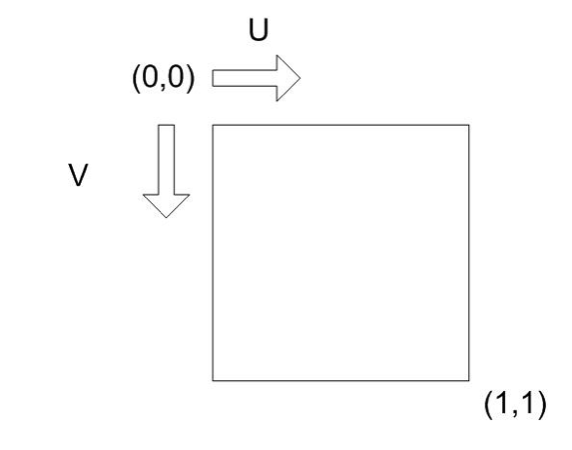
\includegraphics[width=1.5in]{images/terrain_uv}
   \caption{UV coordinates} \cite{TerrainUVs}
 \end{figure}

If we presume that a square texture is to cover the terrain once in its entirety, computing the UV-coordinates for each vertex becomes quite simple. Taking the x (or z) value of a vertex and dividing it by the total width of the terrain, gives us the UV coordinates of that vertex. The first vertex will then have a UV coordinate of 0 (0/width) and the outer most vertext a UV coordinate of 1 (width/width), with everything else in between. Having caculated the UVs, the terrain can then be textured in the pixel shader stage.

\section{Animation}
For animating the grass blades, a simulation of wind is used to achieve a realistic look. In order to maximize the interactivity, the user should be able to influence wind speed and direction. 

In general, the wind simulation consists of two components:

\begin{description}
  \item[Vertex displacement] \hfill \\
  This components takes care of simulation the effect of wind hitting a single blade, which displaces the mesh.
  \item[Wind field simulation] \hfill \\
  To simulate the effect of wind over a field of grass, a 2D wind field is used.
\end{description}

\subsection{Vertex displacement}
The grass blade vertex displacement depends on two components. The wind that is currently hitting the grass blade affects the displacement - however, if you only use this factor, then the animation will look very shallow and unrealistic. If you watch grass blades reacting to wind in real life, you can see that they don't smoothly bend in all directions over and over again, instead, they jitter, they oscillate.

The horizontal vertex displacement depending on the wind can easily be implemented by
\begin{equation}
Position.xz = WindVector.xy * WindCoEff
\end{equation}
where WindVector is the vector of the wind that is hitting the grass blade in the current position. The WindCoEff is a factor that is introduced while generating the grass vertices. This is based upon the idea that the grass blade moves a lot at the top, but does not move at all at the root. Therefore the WindCoEff would be 0 in the root and then increases until it hits 1 at the top.

The vertical vertex displacement is then calculated by
\begin{equation}
Position.y = WindForce * WindCoEff
\end{equation}
where WindForce is the length of the WindVector. This is needed to prevent the grass blade from stretching. If we displace vertices, we need to make sure that the overall length of the grass blade is still the same afterwards. Otherwise, the grass blade would get longer or shorter depending on the wind.

The oscillation factor can then be computed by
\begin{center}
\begin{align*}
LerpCoEff = \frac{sin(oS * dT + sinSkewCoEff) + 1.0)}{2}
\end{align*}
\end{center}
where the oscillationStrength (oS) is just a defined factor, which in our case is 5. The deltaTime (dT) is the time in milliseconds that elapsed since the last frame (usual deltaTime used in games). The sinSkewCoEff is derived from the random value we computed in chapter "Randomization". It's used to differentiate the oscillation pattern for each grass blade which makes the scene look much more natural. And then the value we get out of the sin (-1 to 1) is brought between 0 and 1.

 \begin{figure}[ht]
   \centering
   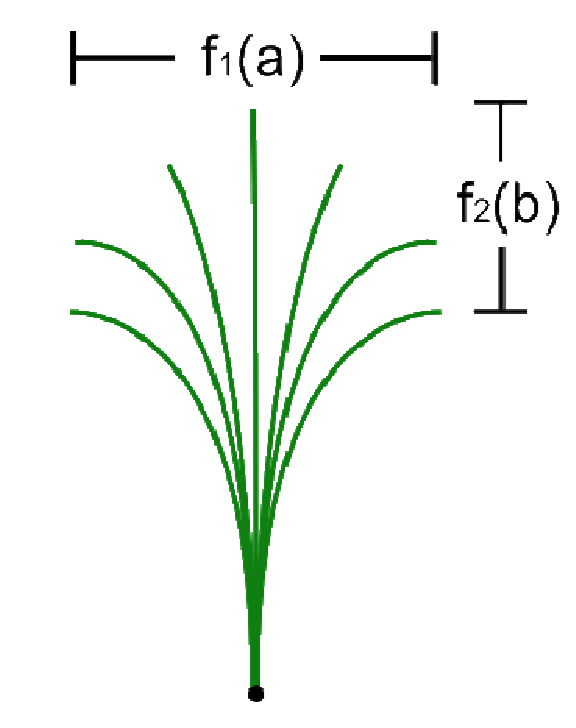
\includegraphics[width=1.75in]{images/oscillation}
   \caption{Oscillation range of a grass blade} \cite{EddieLee}
 \end{figure}

This oscillation factor now has to be used to infuence the WindVector that is reponsible for the vertex displacement. This is done using the formula below.
\begin{equation}
\begin{split}
WindVector = lerp(WindVector * (1.0 - oscillateDelta), \\ 
WindVector * (1.0 + oscillateDelta), LerpCoEff)
\end{split}
\end{equation}
In essence, this opens up a range depending on the current WindVector and the oscillation constant called oscillateDelta, which in our case is "0.35". The final position to take in the range is then defined by our LerpCoEff.

As a sidenote, it can be useful to further randomize the wind by adding a small random direction or force.

\subsection{Wind field simulation}
While the vertex displacement focuses on the impact of wind on a single grass blade indepedently, a system has to be used in order to get all grass blades into the same world - i.e. reacting to the same wind conditions. Since we have a grass field that consists of grass patches, it makes a lot of sense to build a wind field that contains of wind vectors. One wind vector is then assigned to one grass patch and it will be responsible for the wind impact in this grass patch. This wind vector is basically the wind vector that is described in the vertex displacement.

 \begin{figure}[ht]
   \centering
   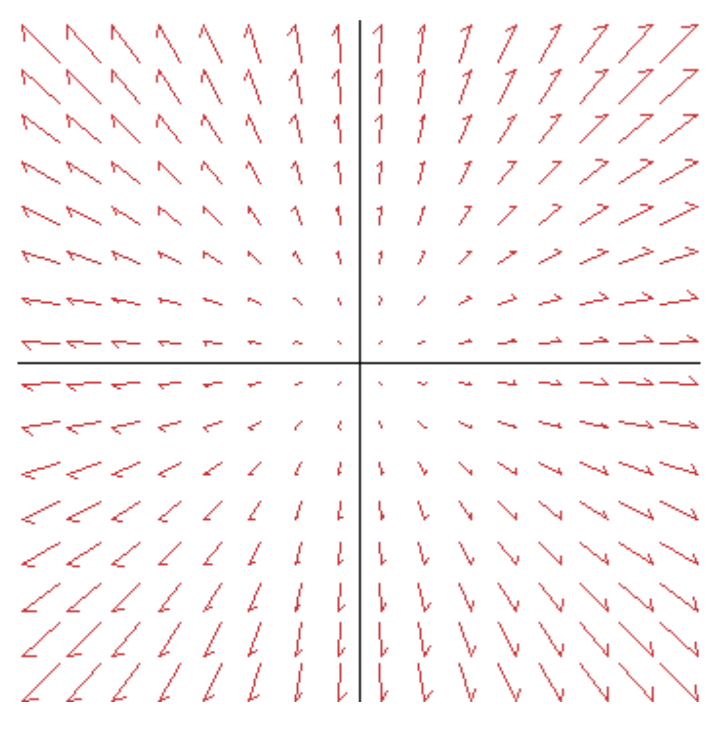
\includegraphics[width=1.75in]{images/windField}
   \caption{Example wind vector field} \cite{EddieLee}
 \end{figure}
 
It is then possible to blow wind into one direction, so that the bottom vectors will have increased velocity and acceleration. For each frame, the acceleration of each vector has to be dampened to avoid ever-increasing wind. Then, each vector has to be diffused with neighbour vectors, which means that the vectors will influence each other and the wind will travel from the bottom upwards. To calculate the current velocity of a wind vector, apply Euler Integration for each wind velocity vector.

\begin{center}
\begin{align}
Velocity = Velocity + Acceleration * dT
\end{align}
\end{center}

One problem still remains: We only have one wind vector per grass patch, meaning that all grass blades inside the patch will move the same way. There will also be breaks of the movement because the wind will change abruptly between patches. To solve this, interpolate linearly between the wind vectors to compute the velocity for the current root.

 \begin{figure}[ht]
   \centering
   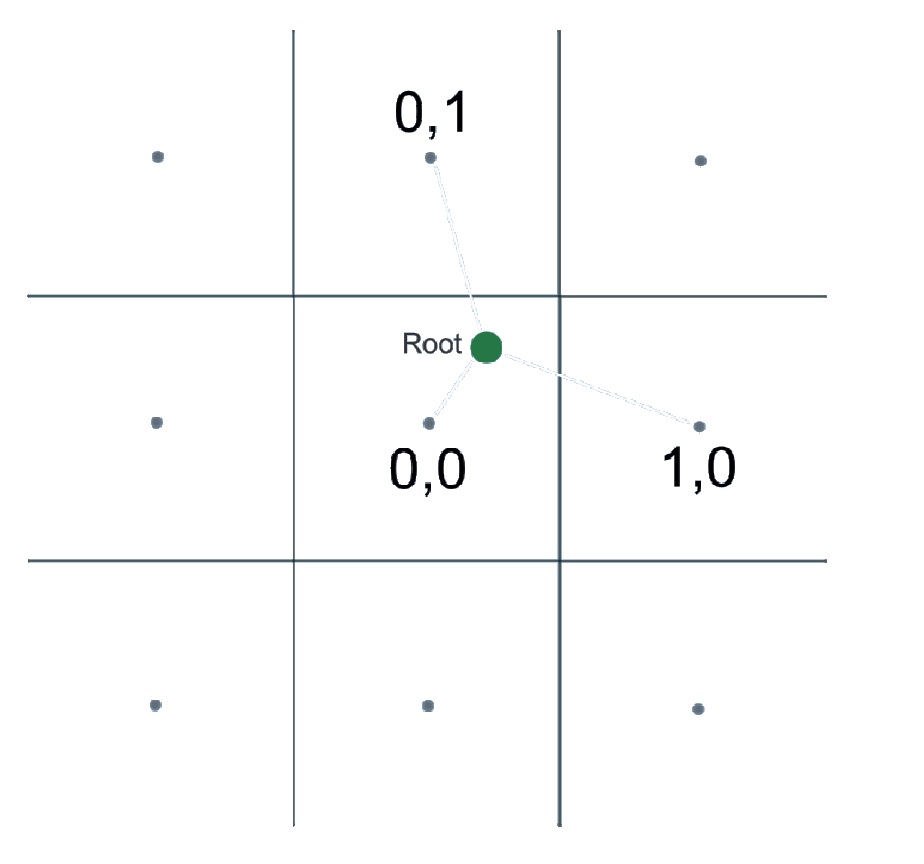
\includegraphics[width=1.75in]{images/wind_field_interpolation}
   \caption{Interpolation of wind vectors} \cite{EddieLee}
 \end{figure}

This will ensure a smooth transition between wind vectors and therefore results in a more realistically looking grass field.

\section{Benchmarks}
We kept randomized values to a minimum to avoid variations in the scene and to have a baseline. All tests were mainly done on the following two systems.

\begin{flushleft}
\begin{description}
  \item[System 1 (Desktop)] \hfill \\
  CPU: Intel Xeon E5-1230v3 \linebreak
  RAM: 8GB DDR3-1333 \linebreak
  GPU: nVidia GeForce GTX 780
  \item[System 2 (Notebook)] \hfill \\
  CPU: Intel Core I7-4980HQ \linebreak
  RAM: 16GB DDR3-1333 \linebreak
  GPU: Intel Iris Pro
\end{description}
\end{flushleft}

Our first benchmark is run on System 1 and is running Ultra-HD resolution to prevent flickering. It has 5 levels of detail defined and contains a quarter million grass blades.

 \begin{figure}[ht]
   \centering
   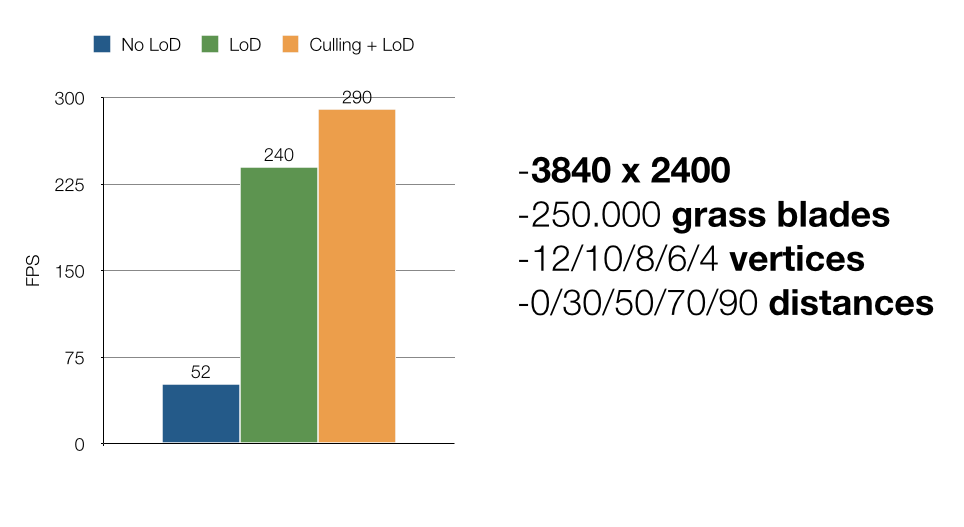
\includegraphics[width=3.6in]{images/benchmark1}
   \caption{Benchmark on System 1}
 \end{figure}    

As you can see, without level of detail, the performance is abysmal. However, when adding level of detail the performance skyrockets, FPS being nearly 4 times as high. At the same time, it is nearly indistinguishable. Further adding culling does not impact the framerate as much, but it is still very noticeable. It has to be kept in mind that culling adds overhead if nothing can be culled, but can improve performance by a lot if many patches can be culled.

We've run the same benchmark with only Full-HD resolution on System 2, these are the results:

 \begin{figure}[ht]
   \centering
   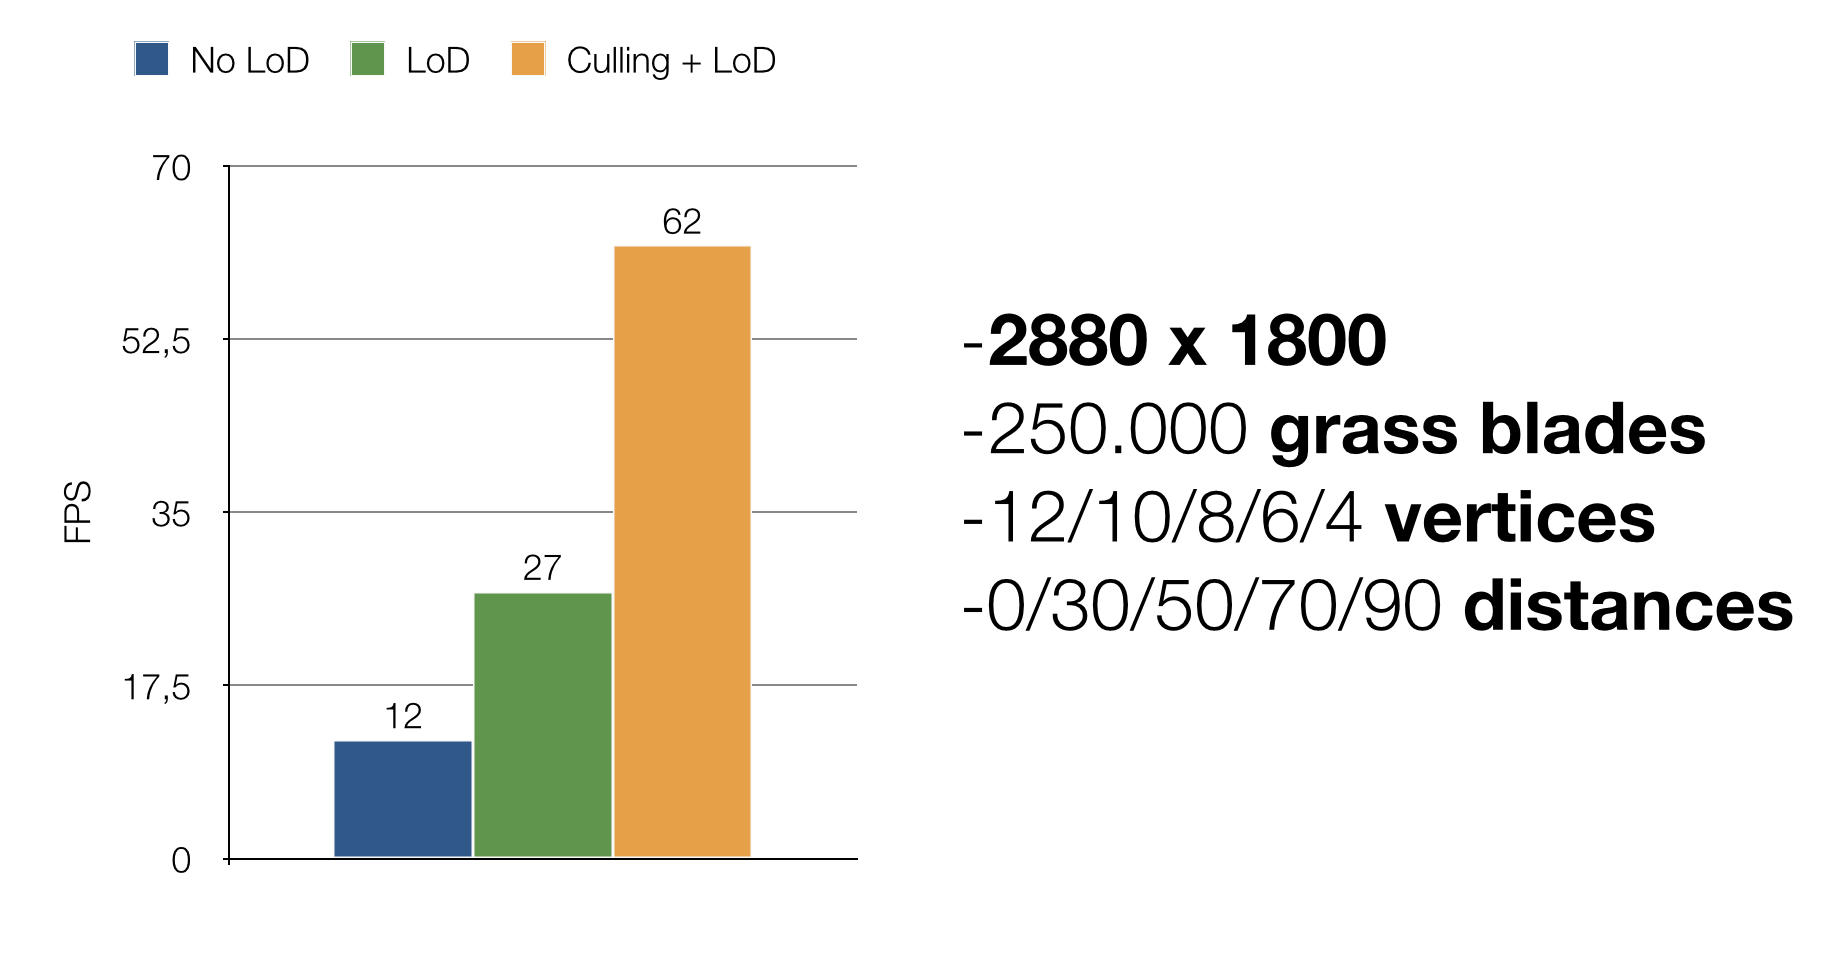
\includegraphics[width=3.6in]{images/benchmark2}
   \caption{Benchmark on System 2}
 \end{figure}    

As can be seen, performance improvements are quite similar - culling is bringing a bigger performance boost, though. The most important thing to note here is that System 2 is a rather low-performance system in terms of GPU performance. Being an integrated graphics chip, it's still possible to run the application with more than 60 FPS.

\section{Shortcomings and improvements}

As shown in the section "Benchmarks", this approach does not need high-end processing power as of todays standards. Using a quarter million grass blades, the implementation can be run on integrated graphics cards on Notebooks with 60 FPS.

The main visual problem is flickering. Using native resolution of displays and no anti-aliasing, the thin blades cause a lot of flickering in the distance - even when using the tricks described in the paper to minimize it. However, when rendered on a high PPI screen or by using techniques like Downsampling, flickering vanishes very fast.

 \begin{figure}[ht]
   \centering
   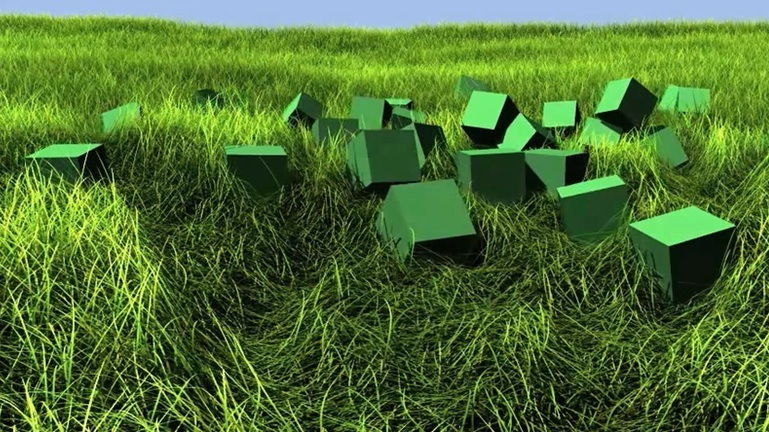
\includegraphics[width=3.0in]{images/turf_effects}
   \caption{Nvidia Turf Effects Demonstration} \cite{NvidiaTurfEffects} \footnote{https://developer.nvidia.com/turfeffects}
 \end{figure}    

To conclude, using geometry shaders to render grass in real time applications is very possible and does not require high-end hardware. Nvidia already released a solution as part of their Gameworks framework, which is called Nvidia Turf Effects and features massive grass simulations with physical interaction.

\bibliographystyle{acmsiggraph}
\bibliography{template}
\end{document}
